% 图 76.2 —— 由 `checks/emit_hand.py` 自动拼出（probe 精测 + prims2 图元分解）
%%
% ⚠ 这是**稿子不是成品**：跑 `checks/checkhand.py 76.2` 看指标 + 看叠合图。
%%
%% ⚠ 待核：
%   · 本图 probe 报出阴影族 2 个 —— **本脚本不生成阴影**（要照原书手写）；prims2 的 strokes 里可能含阴影线，核对时留意别画重
%   · 可疑字形 4 项（空心圈 ⊙ 常被认成字母 o）—— 见文件末
%%
\documentclass[12pt]{standalone}
\usepackage{fontspec}
\setsansfont{Arial}
\newfontfamily\mfallback{DejaVu Sans}
\usepackage{tikz}
\begin{document}
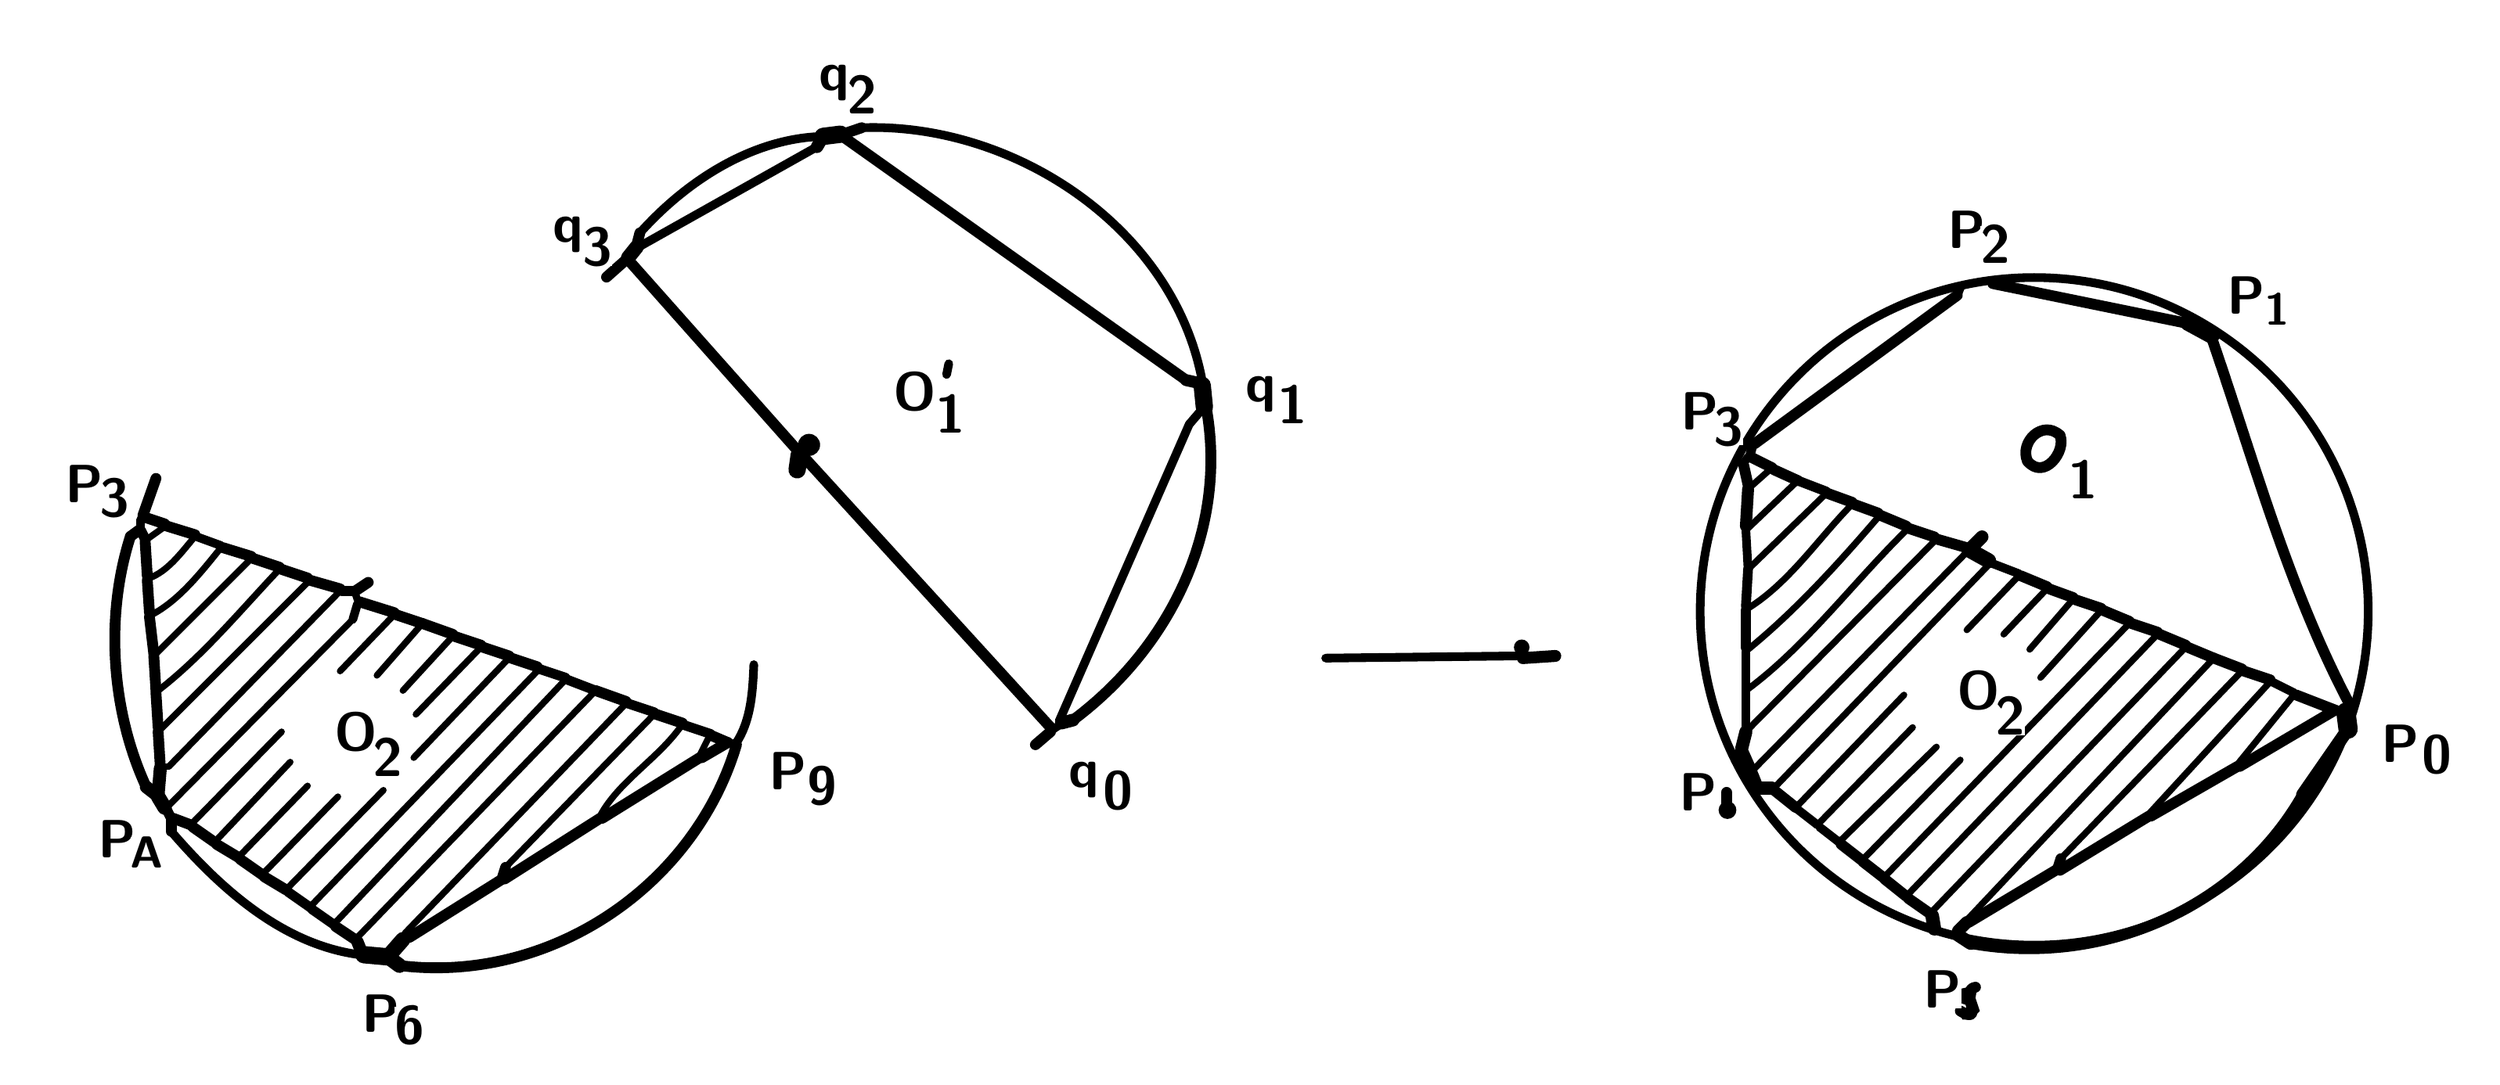
\begin{tikzpicture}[x=1pt, y=-1pt, line width=4.0pt, line cap=round, line join=round]

  %% ════ 填充区（prims2 的 fills）════
  \fill (903.0,445.0) -- (894.0,447.0) -- (894.0,453.0) -- (900.0,455.0) -- (898.0,458.0) -- (894.0,457.0) -- (896.0,461.0) -- (900.0,461.0) -- (904.0,457.0) -- (902.0,451.0) -- cycle;

  %% ════ 直线段（prims2 的 strokes）════
  \draw[line width=3.0pt] (908.0,251.0) -- (809.0,354.0);
  \draw[line width=6.7pt] (66.0,363.0) -- (63.0,358.0);
  \draw[line width=5.0pt] (172.0,273.0) -- (156.0,268.0);
  \draw[line width=5.5pt] (797.0,216.0) -- (796.0,233.0);
  \draw[line width=7.5pt] (1011.0,145.0) -- (1000.0,139.0);
  \draw[line width=4.0pt] (55.0,234.0) -- (55.0,230.0);
  \draw[line width=5.0pt] (62.0,211.0) -- (56.0,228.0);
  \draw[line width=3.0pt] (238.0,300.0) -- (134.0,408.0);
  \draw[line width=6.6pt] (280.0,109.0) -- (284.0,104.0);
  \draw[line width=5.0pt] (910.0,121.0) -- (998.0,139.0);
  \draw[line width=3.0pt] (840.0,378.0) -- (884.0,335.0);
  \draw[line width=3.0pt] (898.0,281.0) -- (921.0,257.0);
  \draw[line width=3.0pt] (211.0,290.0) -- (182.0,320.0);
  \draw[line width=4.0pt] (428.0,158.0) -- (427.0,163.0);
  \draw[line width=3.0pt] (898.0,415.0) -- (1012.0,294.0);
  \draw[line width=4.5pt] (123.0,402.0) -- (133.0,409.0);
  \draw[line width=3.0pt] (946.0,268.0) -- (927.0,290.0);
  \draw[line width=5.0pt] (106.0,247.0) -- (93.0,243.0);
  \draw[line width=5.0pt] (225.0,293.0) -- (213.0,289.0);
  \draw[line width=5.0pt] (280.0,110.0) -- (359.0,199.0);
  \draw[line width=5.0pt] (199.0,283.0) -- (185.0,278.0);
  \draw[line width=5.0pt] (133.0,258.0) -- (147.0,262.0);
  \draw[line width=4.0pt] (796.0,235.0) -- (797.0,253.0);
  \draw[line width=7.0pt] (169.0,432.0) -- (176.0,424.0);
  \draw[line width=8.0pt] (169.0,432.0) -- (158.0,431.0);
  \draw[line width=6.8pt] (169.0,432.0) -- (174.4,436.0);
  \draw[line width=5.0pt] (898.0,243.0) -- (884.0,239.0);
  \draw[line width=3.0pt] (65.0,344.0) -- (68.0,344.0);
  \draw[line width=3.0pt] (68.0,344.0) -- (147.0,263.0);
  \draw[line width=3.0pt] (132.0,353.0) -- (101.0,385.0);
  \draw[line width=4.5pt] (144.0,417.0) -- (134.0,410.0);
  \draw[line width=5.0pt] (145.0,418.0) -- (154.0,424.0);
  \draw[line width=5.0pt] (314.0,340.0) -- (326.0,333.0);
  \draw[line width=5.0pt] (285.4,97.6) -- (284.0,103.0);
  \draw[line width=8.0pt] (370.0,53.0) -- (378.0,52.0);
  \draw[line width=5.8pt] (370.0,53.0) -- (367.2,57.8);
  \draw[line width=4.0pt] (367.2,57.8) -- (285.0,104.0);
  \draw[line width=5.0pt] (379.0,53.0) -- (537.6,165.6);
  \draw[line width=5.5pt] (537.6,165.6) -- (544.0,167.0);
  \draw[line width=3.8pt] (795.0,204.0) -- (797.0,201.0);
  \draw[line width=3.8pt] (1073.0,318.0) -- (1075.0,315.0);
  \draw[line width=5.0pt] (1000.0,289.0) -- (1012.0,294.0);
  \draw[line width=5.0pt] (279.0,314.0) -- (265.0,309.0);
  \draw[line width=5.0pt] (787.0,361.0) -- (787.0,356.0);
  \draw[line width=3.0pt] (882.0,411.0) -- (998.0,290.0);
  \draw[line width=5.0pt] (67.0,233.0) -- (80.0,237.0);
  \draw[line width=5.0pt] (475.0,328.0) -- (468.0,334.0);
  \draw[line width=5.0pt] (62.0,309.0) -- (61.0,293.0);
  \draw[line width=3.0pt] (313.0,339.0) -- (317.0,331.0);
  \draw[line width=3.0pt] (883.0,240.0) -- (797.0,327.0);
  \draw[line width=5.0pt] (1068.0,318.0) -- (1050.0,311.0);
  \draw[line width=4.0pt] (1068.0,318.0) -- (1072.0,318.0);
  \draw[line width=5.0pt] (1068.0,318.0) -- (1024.0,344.0);
  \draw[line width=5.0pt] (819.0,363.0) -- (809.0,355.0);
  \draw[line width=3.0pt] (860.0,395.0) -- (972.0,279.0);
  \draw[line width=5.0pt] (59.0,275.0) -- (61.0,292.0);
  \draw[line width=5.0pt] (809.0,207.0) -- (820.0,212.0);
  \draw[line width=3.0pt] (982.0,366.0) -- (1038.0,305.0);
  \draw[line width=5.0pt] (120.0,253.0) -- (132.0,257.0);
  \draw[line width=4.9pt] (222.0,395.0) -- (223.4,390.6);
  \draw[line width=3.0pt] (223.4,390.6) -- (291.0,321.0);
  \draw[line width=5.0pt] (90.0,380.0) -- (100.0,386.0);
  \draw[line width=3.0pt] (873.0,326.0) -- (830.0,370.0);
  \draw[line width=3.0pt] (171.0,275.0) -- (147.0,300.0);
  \draw[line width=4.5pt] (251.0,303.0) -- (239.0,299.0);
  \draw[line width=4.3pt] (799.0,196.0) -- (798.0,200.0);
  \draw[line width=5.0pt] (960.0,271.0) -- (948.0,267.0);
  \draw[line width=4.0pt] (1049.0,310.0) -- (1039.0,305.0);
  \draw[line width=5.7pt] (157.0,430.0) -- (155.0,425.0);
  \draw[line width=3.0pt] (64.0,327.0) -- (132.0,259.0);
  \draw[line width=5.0pt] (361.0,201.0) -- (475.0,326.0);
  \draw[line width=3.0pt] (224.0,295.0) -- (181.0,340.0);
  \draw[line width=4.7pt] (67.0,364.0) -- (69.0,368.0);
  \draw[line width=4.0pt] (690.0,293.0) -- (602.0,294.0);
  \draw[line width=3.0pt] (798.0,215.0) -- (807.0,207.0);
  \draw[line width=5.0pt] (212.0,288.0) -- (200.0,284.0);
  \draw[line width=5.5pt] (708.0,293.0) -- (693.0,294.0);
  \draw[line width=5.0pt] (305.0,324.0) -- (293.0,320.0);
  \draw[line width=5.0pt] (185.0,278.0) -- (173.0,274.0);
  \draw[line width=3.0pt] (185.0,278.0) -- (164.0,302.0);
  \draw[line width=5.0pt] (859.0,395.0) -- (850.0,388.0);
  \draw[line width=5.0pt] (101.0,387.0) -- (111.0,394.0);
  \draw[line width=3.0pt] (167.0,355.0) -- (123.0,400.0);
  \draw[line width=5.0pt] (858.0,228.0) -- (870.0,233.0);
  \draw[line width=7.0pt] (908.0,249.0) -- (899.0,244.0);
  \draw[line width=3.0pt] (58.0,239.0) -- (65.0,234.0);
  \draw[line width=5.0pt] (63.0,326.0) -- (62.0,310.0);
  \draw[line width=5.0pt] (797.0,214.0) -- (795.0,205.0);
  \draw[line width=3.0pt] (915.0,283.0) -- (934.0,263.0);
  \draw[line width=5.9pt] (485.4,322.6) -- (480.0,324.0);
  \draw[line width=5.0pt] (238.0,298.0) -- (226.0,294.0);
  \draw[line width=3.0pt] (869.0,311.0) -- (820.0,362.0);
  \draw[line width=5.0pt] (58.0,258.0) -- (59.0,273.0);
  \draw[line width=3.0pt] (112.0,393.0) -- (146.0,358.0);
  \draw[line width=6.0pt] (796.0,328.0) -- (794.0,336.0);
  \draw[line width=5.0pt] (1025.0,299.0) -- (1012.0,294.0);
  \draw[line width=6.0pt] (63.0,357.0) -- (64.0,345.0);
  \draw[line width=3.0pt] (278.0,316.0) -- (177.0,421.0);
  \draw[line width=6.0pt] (808.0,354.0) -- (802.0,354.0);
  \draw[line width=5.0pt] (1023.0,344.0) -- (983.0,367.0);
  \draw[line width=5.0pt] (899.0,416.0) -- (939.0,392.0);
  \draw[line width=4.5pt] (292.0,319.0) -- (280.0,315.0);
  \draw[line width=8.0pt] (359.0,200.0) -- (358.0,207.0);
  \draw[line width=3.0pt] (850.0,387.0) -- (895.0,341.0);
  \draw[line width=4.7pt] (57.0,239.0) -- (55.0,235.0);
  \draw[line width=4.0pt] (796.0,309.0) -- (796.0,291.0);
  \draw[line width=4.0pt] (796.0,309.0) -- (796.0,327.0);
  \draw[line width=3.0pt] (90.0,378.0) -- (124.0,342.0);
  \draw[line width=4.0pt] (820.0,364.0) -- (829.0,371.0);
  \draw[line width=5.0pt] (270.0,118.0) -- (279.0,110.0);
  \draw[line width=3.0pt] (799.0,346.0) -- (898.0,245.0);
  \draw[line width=5.0pt] (78.0,371.0) -- (70.0,368.0);
  \draw[line width=8.0pt] (545.0,168.0) -- (546.0,178.0);
  \draw[line width=5.0pt] (154.0,263.0) -- (160.0,259.0);
  \draw[line width=5.0pt] (923.0,256.0) -- (935.0,261.0);
  \draw[line width=5.0pt] (973.0,277.0) -- (961.0,272.0);
  \draw[line width=3.8pt] (479.0,325.0) -- (476.0,327.0);
  \draw[line width=8.9pt] (1073.0,319.0) -- (1074.0,326.8);
  \draw[line width=6.0pt] (1074.0,326.8) -- (1053.0,357.1);
  \draw[line width=6.0pt] (899.8,425.8) -- (894.0,422.0);
  \draw[line width=5.0pt] (870.0,404.0) -- (860.0,396.0);
  \draw[line width=5.0pt] (871.0,405.0) -- (881.0,412.0);
  \draw[line width=4.5pt] (265.0,309.0) -- (252.0,304.0);
  \draw[line width=3.0pt] (265.0,309.0) -- (155.0,423.0);
  \draw[line width=5.0pt] (849.0,387.0) -- (840.0,380.0);
  \draw[line width=3.0pt] (329.0,333.0) -- (326.0,333.0);
  \draw[line width=4.0pt] (155.0,269.0) -- (152.9,276.1);
  \draw[line width=3.0pt] (152.9,276.1) -- (67.0,363.0);
  \draw[line width=4.0pt] (922.0,255.0) -- (909.0,250.0);
  \draw[line width=5.7pt] (801.0,353.0) -- (799.0,348.0);
  \draw[line width=5.0pt] (798.0,201.0) -- (808.0,206.0);
  \draw[line width=4.9pt] (940.0,391.0) -- (941.4,386.6);
  \draw[line width=3.0pt] (941.4,386.6) -- (1024.0,301.0);
  \draw[line width=7.0pt] (794.0,338.0) -- (798.0,347.0);
  \draw[line width=4.5pt] (318.0,329.0) -- (306.0,325.0);
  \draw[line width=5.0pt] (883.0,238.0) -- (871.0,234.0);
  \draw[line width=5.0pt] (941.0,392.0) -- (982.0,367.0);
  \draw[line width=5.0pt] (54.0,235.0) -- (50.2,237.8);
  \draw[line width=5.9pt] (57.5,353.5) -- (62.0,357.0);
  \draw[line width=5.0pt] (319.0,330.0) -- (326.0,333.0);
  \draw[line width=3.0pt] (120.0,328.0) -- (79.0,370.0);
  \draw[line width=5.0pt] (64.0,344.0) -- (63.0,328.0);
  \draw[line width=5.0pt] (313.0,340.0) -- (268.0,368.0);
  \draw[line width=5.0pt] (223.0,396.0) -- (267.0,368.0);
  \draw[line width=5.0pt] (58.0,256.0) -- (57.0,240.0);
  \draw[line width=5.0pt] (1038.0,304.0) -- (1026.0,300.0);
  \draw[line width=3.0pt] (832.0,219.0) -- (797.0,253.0);
  \draw[line width=4.5pt] (820.0,212.0) -- (833.0,217.0);
  \draw[line width=3.0pt] (820.0,212.0) -- (797.0,234.0);
  \draw[line width=3.0pt] (960.0,272.0) -- (932.0,303.0);
  \draw[line width=5.0pt] (222.0,396.0) -- (179.0,423.0);
  \draw[line width=3.0pt] (145.0,416.0) -- (251.0,304.0);
  \draw[line width=6.0pt] (900.0,243.0) -- (905.0,238.0);
  \draw[line width=5.0pt] (986.0,282.0) -- (974.0,278.0);
  \draw[line width=5.0pt] (69.0,369.0) -- (69.0,374.0);
  \draw[line width=3.0pt] (1049.0,311.0) -- (1023.0,343.0);
  \draw[line width=5.0pt] (987.0,283.0) -- (999.0,288.0);
  \draw[line width=4.5pt] (797.0,253.0) -- (796.0,270.0);
  \draw[line width=4.0pt] (479.0,323.0) -- (539.0,186.0);
  \draw[line width=4.0pt] (539.0,186.0) -- (545.0,179.0);
  \draw[line width=3.0pt] (871.0,403.0) -- (986.0,283.0);
  \draw[line width=5.0pt] (834.0,218.0) -- (845.0,222.0);
  \draw[line width=5.0pt] (112.0,395.0) -- (122.0,401.0);
  \draw[line width=3.0pt] (176.0,309.0) -- (198.0,285.0);
  \draw[line width=5.0pt] (387.8,49.0) -- (379.0,52.0);
  \draw[line width=5.0pt] (79.0,372.0) -- (89.0,379.0);
  \draw[line width=5.0pt] (57.0,229.0) -- (66.0,232.0);
  \draw[line width=3.4pt] (154.0,264.0) -- (155.0,267.0);
  \draw[line width=5.0pt] (796.0,272.0) -- (796.0,289.0);
  \draw[line width=5.7pt] (898.0,416.0) -- (894.0,420.0);
  \draw[line width=5.0pt] (800.0,195.0) -- (893.6,126.4);
  \draw[line width=3.9pt] (893.6,126.4) -- (895.0,123.0);
  \draw[line width=5.0pt] (153.0,263.0) -- (148.0,263.0);
  \draw[line width=3.0pt] (105.0,249.0) -- (62.0,292.0);
  \draw[line width=4.0pt] (839.0,379.0) -- (830.0,372.0);
  \draw[line width=6.3pt] (882.0,413.0) -- (883.0,419.0);
  \draw[line width=5.0pt] (119.0,252.0) -- (107.0,248.0);
  \draw[line width=4.0pt] (92.0,242.0) -- (81.0,238.0);
  \draw[line width=5.0pt] (857.0,227.0) -- (846.0,223.0);
  \draw[line width=5.0pt] (936.0,262.0) -- (947.0,266.0);

  %% ════ 曲线（prims2 的 curves —— 三段式，坐标同为 (y,x)）════
  \draw[line width=5.0pt] (174.4,436.0) .. controls (244.0,444.6) and (310.6,399.3) .. (330.0,334.0);
  \draw[line width=4.0pt] (370.0,53.0) .. controls (338.0,53.8) and (307.6,72.8) .. (285.4,97.6);
  \draw[line width=3.0pt] (92.0,243.0) .. controls (82.8,254.4) and (72.7,267.3) .. (60.0,274.0);
  \draw[line width=3.0pt] (267.0,367.0) .. controls (275.3,351.3) and (293.4,340.7) .. (304.0,326.0);
  \draw[line width=3.0pt] (870.0,235.0) .. controls (845.5,259.1) and (823.6,288.7) .. (796.0,309.0);
  \draw[line width=4.0pt] (338.0,297.0) .. controls (337.5,309.6) and (336.7,322.6) .. (330.0,333.0);
  \draw[line width=5.0pt] (547.0,179.0) .. controls (556.7,234.6) and (530.5,288.9) .. (485.4,322.6);
  \draw[line width=3.0pt] (797.0,271.0) .. controls (815.8,259.3) and (829.2,239.2) .. (844.0,224.0);
  \draw[line width=5.0pt] (895.0,457.0) .. controls (907.0,464.1) and (894.2,447.0) .. (902.0,446.0);
  \draw[line width=5.0pt] (1053.0,357.1) .. controls (1023.0,410.0) and (960.0,436.8) .. (899.8,425.8);
  \draw[line width=5.0pt] (1011.0,146.0) .. controls (1030.5,202.5) and (1046.1,260.6) .. (1074.0,314.0);
  \draw[line width=5.0pt] (50.2,237.8) .. controls (38.4,274.6) and (41.3,318.4) .. (57.5,353.5);
  \draw[line width=3.0pt] (59.0,257.0) .. controls (67.2,254.0) and (73.4,245.7) .. (79.0,239.0);
  \draw[line width=4.0pt] (69.0,374.0) .. controls (92.4,401.2) and (121.0,426.4) .. (156.0,431.0);
  \draw[line width=4.0pt] (545.0,166.0) .. controls (531.9,95.1) and (457.9,46.4) .. (387.8,49.0);
  \draw[line width=3.0pt] (118.0,254.0) .. controls (100.7,272.4) and (83.1,293.5) .. (63.0,309.0);
  \draw[line width=3.0pt] (797.0,290.0) .. controls (818.9,272.1) and (838.7,250.3) .. (857.0,229.0);
  \draw[line width=5.0pt] (926.0,203.0) .. controls (922.2,194.2) and (933.0,183.6) .. (941.0,191.1);
  \draw[line width=5.0pt] (941.0,191.1) .. controls (944.0,198.5) and (933.6,212.1) .. (926.0,203.0);

  %% ════ 圆 / 椭圆（probe 精测）════
  \draw (929.1,272.4) circle (154.2);

  %% ════ 实心点 ════
  \fill (363.5,195.5) circle (5.1);
  \fill (692.5,289.0) circle (3.6);
  \fill (787.5,364.2) circle (4.1);

  %% ════ 标签（probe 直接给的 \node 行）════
  %% ⚠ 全部补了 fill=white：文字在最上层，否则与曲线交叉干扰
     \node[anchor=center,inner sep=0pt,fill=white,font=\fontsize{32.0}{40.0}\selectfont] at (375.1,28.4) {\textsf{\textbf{\textit{q}}}};   % box(365,15,18,23)
     \node[anchor=center,inner sep=0pt,fill=white,font=\fontsize{23.6}{29.6}\selectfont] at (388.1,33.9) {\textsf{\textbf{2}}};   % box(382,25,11,17)
     \node[anchor=center,inner sep=0pt,fill=white,font=\fontsize{29.2}{36.4}\selectfont] at (897.9,96.0) {\textsf{\textbf{\textit{P}}}};   % box(887,84,18,22)
     \node[anchor=center,inner sep=0pt,fill=white,font=\fontsize{32.0}{40.0}\selectfont] at (252.1,98.4) {\textsf{\textbf{\textit{q}}}};   % box(242,85,18,23)
     \node[anchor=center,inner sep=0pt,fill=white,font=\fontsize{23.6}{29.6}\selectfont] at (911.1,102.9) {\textsf{\textbf{2}}};   % box(905,94,11,17)
     \node[anchor=center,inner sep=0pt,fill=white,font=\fontsize{23.0}{28.7}\selectfont] at (265.9,104.1) {\textsf{\textbf{3}}};   % box(260,95,11,17)
     \node[anchor=center,inner sep=0pt,fill=white,font=\fontsize{29.8}{37.3}\selectfont] at (1027.0,126.5) {\textsf{\textbf{\textit{P}}}};   % box(1016,114,18,23)
     \node[anchor=center,inner sep=0pt,fill=white,font=\fontsize{19.9}{24.9}\selectfont] at (1041.3,132.8) {\textsf{\textbf{1}}};   % box(1036,125,6,15)
     \node[anchor=center,inner sep=0pt,fill=white,font=\fontsize{30.4}{38.0}\selectfont] at (412.3,171.0) {\textsf{\textbf{\textit{O}}}};   % box(400,159,22,22)
     \node[anchor=center,inner sep=0pt,fill=white,font=\fontsize{32.0}{40.0}\selectfont] at (572.1,172.4) {\textsf{\textbf{\textit{q}}}};   % box(562,159,18,23)
     \node[anchor=center,inner sep=0pt,fill=white,font=\fontsize{29.2}{36.4}\selectfont] at (774.9,180.0) {\textsf{\textbf{\textit{P}}}};   % box(764,168,18,22)
     \node[anchor=center,inner sep=0pt,fill=white,font=\fontsize{23.0}{28.7}\selectfont] at (586.7,176.9) {\textsf{\textbf{1}}};   % box(580,169,8,15)
     \node[anchor=center,inner sep=0pt,fill=white,font=\fontsize{23.7}{29.7}\selectfont] at (428.8,181.4) {\textsf{\textbf{1}}};   % box(422,173,8,16)
     \node[anchor=center,inner sep=0pt,fill=white,font=\fontsize{23.0}{28.7}\selectfont] at (787.9,187.1) {\textsf{\textbf{3}}};   % box(782,178,11,17)
     \node[anchor=center,inner sep=0pt,fill=white,font=\fontsize{29.8}{37.3}\selectfont] at (29.0,213.5) {\textsf{\textbf{\textit{P}}}};   % box(18,201,18,23)
     \node[anchor=center,inner sep=0pt,fill=white,font=\fontsize{23.0}{28.7}\selectfont] at (951.7,211.9) {\textsf{\textbf{1}}};   % box(945,204,8,15)
     \node[anchor=center,inner sep=0pt,fill=white,font=\fontsize{23.0}{28.7}\selectfont] at (42.9,220.1) {\textsf{\textbf{3}}};   % box(37,211,11,17)
     \node[anchor=center,inner sep=0pt,fill=white,font=\fontsize{30.4}{38.0}\selectfont] at (903.3,309.0) {\textsf{\textbf{\textit{O}}}};   % box(891,297,22,22)
     \node[anchor=center,inner sep=0pt,fill=white,font=\fontsize{23.6}{29.6}\selectfont] at (918.1,320.9) {\textsf{\textbf{2}}};   % box(912,312,11,17)
     \node[anchor=center,inner sep=0pt,fill=white,font=\fontsize{30.4}{38.0}\selectfont] at (154.3,328.0) {\textsf{\textbf{\textit{O}}}};   % box(142,316,22,22)
     \node[anchor=center,inner sep=0pt,fill=white,font=\fontsize{29.8}{37.3}\selectfont] at (1098.0,333.5) {\textsf{\textbf{\textit{P}}}};   % box(1087,321,18,23)
     \node[anchor=center,inner sep=0pt,fill=white,font=\fontsize{24.9}{31.1}\selectfont] at (1115.1,338.7) {\textsf{\textbf{0}}};   % box(1107,330,12,17)
     \node[anchor=center,inner sep=0pt,fill=white,font=\fontsize{23.6}{29.6}\selectfont] at (169.1,339.9) {\textsf{\textbf{2}}};   % box(163,331,11,17)
     \node[anchor=center,inner sep=0pt,fill=white,font=\fontsize{29.2}{36.4}\selectfont] at (353.9,346.0) {\textsf{\textbf{\textit{P}}}};   % box(343,334,18,22)
     \node[anchor=center,inner sep=0pt,fill=white,font=\fontsize{31.1}{38.9}\selectfont] at (490.5,350.3) {\textsf{\textbf{\textit{q}}}};   % box(481,337,17,23)
     \node[anchor=center,inner sep=0pt,fill=white,font=\fontsize{24.4}{30.5}\selectfont] at (369.4,353.1) {\textsf{\textbf{9}}};   % box(362,344,12,17)
     \node[anchor=center,inner sep=0pt,fill=white,font=\fontsize{29.2}{36.4}\selectfont] at (773.9,356.0) {\textsf{\textbf{\textit{P}}}};   % box(763,344,18,22)
     \node[anchor=center,inner sep=0pt,fill=white,font=\fontsize{24.1}{30.2}\selectfont] at (506.0,355.2) {\textsf{\textbf{0}}};   % box(498,347,12,16)
     \node[anchor=center,inner sep=0pt,fill=white,font=\fontsize{29.8}{37.3}\selectfont] at (44.0,377.5) {\textsf{\textbf{\textit{P}}}};   % box(33,365,18,23)
     \node[anchor=center,inner sep=0pt,fill=white,font=\fontsize{19.4}{24.3}\selectfont] at (57.8,383.8) {\textsf{\textbf{\textit{A}}}};   % box(50,376,12,15)
     \node[anchor=center,inner sep=0pt,fill=white,font=\fontsize{29.2}{36.4}\selectfont] at (886.9,447.0) {\textsf{\textbf{\textit{P}}}};   % box(876,435,18,22)
     \node[anchor=center,inner sep=0pt,fill=white,font=\fontsize{29.2}{36.4}\selectfont] at (165.9,458.0) {\textsf{\textbf{\textit{P}}}};   % box(155,446,18,22)
     \node[anchor=center,inner sep=0pt,fill=white,font=\fontsize{24.1}{30.1}\selectfont] at (179.1,463.6) {\textsf{\textbf{6}}};   % box(173,454,11,18)

  % 钉死画布：否则超出的图元/控制点会把页面撑大，1:1 回比就失准
  \pgfresetboundingbox
  \path[use as bounding box] (0,0) rectangle (1134,481);
\end{tikzpicture}
\end{document}

% ⚠ 待核清单（probe 拿不准，人眼过一遍）：
%   · 可疑字形：\node[anchor=center,inner sep=0pt,font=\fontsize{30.4}{38.0}\selectfont] at (412.3,171.0) {\textsf{\textbf{\te
%   · 可疑字形：\node[anchor=center,inner sep=0pt,font=\fontsize{30.4}{38.0}\selectfont] at (903.3,309.0) {\textsf{\textbf{\te
%   · 可疑字形：\node[anchor=center,inner sep=0pt,font=\fontsize{30.4}{38.0}\selectfont] at (154.3,328.0) {\textsf{\textbf{\te
%   · 未识别/跳过：⑤ 跳过/未识别的字形
